\sectionthree{Deterministic Finite State Machines}
\begin{python0}
from solutions import *; clear()
\end{python0}

We need to formalize DFAs.

\begin{defn}
  A \defone{deterministic finite automata}
  (\sidebarskip{16pt}\defone{DFA})
  or a
  \sidebarskip{8pt}\defone{deterministic finite state machine}\sidebarskip{4pt}
  is defined by
  \[
  (\Sigma,Q,q_0,F,\delta)
  \]
  where
  \begin{tightlist}
  \item $\Sigma$ is a finite set called the
    \defone{alphabet}
  \item $Q$ is a set of \defone{states}
  \item $q_0 \in Q$ is the
    \defone{start state}
    or
    \sidebarskip{12pt}\defone{initial state}
  \item $F \subseteq Q$ is the set of 
    \defone{accept states}
    or
    \sidebarskip{18pt}\defone{final states}
  \item $\delta : Q \times \Sigma \rightarrow Q$ is the
    \defone{transition function}.
  \end{tightlist}
  In this case we will say that $M$ is defined over $\Sigma$.
\end{defn}

Note: In some books the ingredients
for a DFA is listed in this order $(Q, \Sigma, \delta, q_0, F)$
instead where the set of states come first.

\begin{ex}
  Write down the formal definition of the DFA from the
  state diagram in the previous section.

\begin{center}
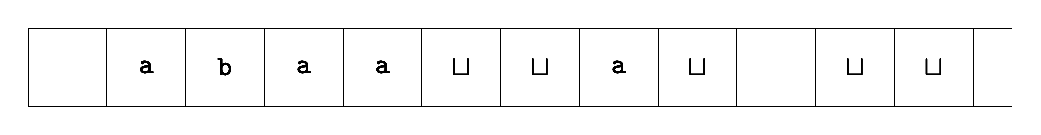
\begin{tikzpicture}

\draw (0.49999999999999994, 0.49999999999999994)
  node[draw, line width=0.01cm, , color=black,
       rounded corners=0cm, inner sep=0cm] {

\begin{minipage}[t][1.0cm]{1.0cm}
\mbox{}

\end{minipage}

};\draw (0.49999999999999994, 0.49999999999999994) node[color=black] {\texttt{\DOLLAR}};
\draw (1.5, 0.49999999999999994)
  node[draw, line width=0.01cm, , color=black,
       rounded corners=0cm, inner sep=0cm] {

\begin{minipage}[t][1.0cm]{1.0cm}
\mbox{}

\end{minipage}

};\draw (1.5, 0.49999999999999994) node[color=black] {\texttt{a}};
\draw (2.5, 0.49999999999999994)
  node[draw, line width=0.01cm, , color=black,
       rounded corners=0cm, inner sep=0cm] {

\begin{minipage}[t][1.0cm]{1.0cm}
\mbox{}

\end{minipage}

};\draw (2.5, 0.49999999999999994) node[color=black] {\texttt{b}};
\draw (3.5, 0.49999999999999994)
  node[draw, line width=0.01cm, , color=black,
       rounded corners=0cm, inner sep=0cm] {

\begin{minipage}[t][1.0cm]{1.0cm}
\mbox{}

\end{minipage}

};\draw (3.5, 0.49999999999999994) node[color=black] {\texttt{a}};
\draw (4.5, 0.49999999999999994)
  node[draw, line width=0.01cm, , color=black,
       rounded corners=0cm, inner sep=0cm] {

\begin{minipage}[t][1.0cm]{1.0cm}
\mbox{}

\end{minipage}

};\draw (4.5, 0.49999999999999994) node[color=black] {\texttt{a}};
\draw (5.5, 0.49999999999999994)
  node[draw, line width=0.01cm, , color=black,
       rounded corners=0cm, inner sep=0cm] {

\begin{minipage}[t][1.0cm]{1.0cm}
\mbox{}

\end{minipage}

};\draw (5.5, 0.49999999999999994) node[color=black] {\texttt{$\sqcup$}};
\draw (6.5, 0.49999999999999994)
  node[draw, line width=0.01cm, , color=black,
       rounded corners=0cm, inner sep=0cm] {

\begin{minipage}[t][1.0cm]{1.0cm}
\mbox{}

\end{minipage}

};\draw (6.5, 0.49999999999999994) node[color=black] {\texttt{$\sqcup$}};
\draw (7.5, 0.49999999999999994)
  node[draw, line width=0.01cm, , color=black,
       rounded corners=0cm, inner sep=0cm] {

\begin{minipage}[t][1.0cm]{1.0cm}
\mbox{}

\end{minipage}

};\draw (7.5, 0.49999999999999994) node[color=black] {\texttt{a}};
\draw (8.5, 0.49999999999999994)
  node[draw, line width=0.01cm, , color=black,
       rounded corners=0cm, inner sep=0cm] {

\begin{minipage}[t][1.0cm]{1.0cm}
\mbox{}

\end{minipage}

};\draw (8.5, 0.49999999999999994) node[color=black] {\texttt{$\sqcup$}};
\draw (9.5, 0.49999999999999994)
  node[draw, line width=0.01cm, , color=black,
       rounded corners=0cm, inner sep=0cm] {

\begin{minipage}[t][1.0cm]{1.0cm}
\mbox{}

\end{minipage}

};\draw (9.5, 0.49999999999999994) node[color=black] {\texttt{$\EOT$}};
\draw (10.5, 0.49999999999999994)
  node[draw, line width=0.01cm, , color=black,
       rounded corners=0cm, inner sep=0cm] {

\begin{minipage}[t][1.0cm]{1.0cm}
\mbox{}

\end{minipage}

};\draw (10.5, 0.49999999999999994) node[color=black] {\texttt{$\sqcup$}};
\draw (11.5, 0.49999999999999994)
  node[draw, line width=0.01cm, , color=black,
       rounded corners=0cm, inner sep=0cm] {

\begin{minipage}[t][1.0cm]{1.0cm}
\mbox{}

\end{minipage}

};\draw (11.5, 0.49999999999999994) node[color=black] {\texttt{$\sqcup$}};
\draw (0.49999999999999994, 0.49999999999999994)
  node[draw, line width=0.01cm, , color=black,
       rounded corners=0cm, inner sep=0cm] {

\begin{minipage}[t][1.0cm]{1.0cm}
\mbox{}

\end{minipage}

};\draw (0.49999999999999994, 0.49999999999999994) node[color=black] {\texttt{\DOLLAR}};
\draw (1.5, 0.49999999999999994)
  node[draw, line width=0.01cm, , color=black,
       rounded corners=0cm, inner sep=0cm] {

\begin{minipage}[t][1.0cm]{1.0cm}
\mbox{}

\end{minipage}

};\draw (1.5, 0.49999999999999994) node[color=black] {\texttt{a}};
\draw (2.5, 0.49999999999999994)
  node[draw, line width=0.01cm, , color=black,
       rounded corners=0cm, inner sep=0cm] {

\begin{minipage}[t][1.0cm]{1.0cm}
\mbox{}

\end{minipage}

};\draw (2.5, 0.49999999999999994) node[color=black] {\texttt{b}};
\draw (3.5, 0.49999999999999994)
  node[draw, line width=0.01cm, , color=black,
       rounded corners=0cm, inner sep=0cm] {

\begin{minipage}[t][1.0cm]{1.0cm}
\mbox{}

\end{minipage}

};\draw (3.5, 0.49999999999999994) node[color=black] {\texttt{a}};
\draw (4.5, 0.49999999999999994)
  node[draw, line width=0.01cm, , color=black,
       rounded corners=0cm, inner sep=0cm] {

\begin{minipage}[t][1.0cm]{1.0cm}
\mbox{}

\end{minipage}

};\draw (4.5, 0.49999999999999994) node[color=black] {\texttt{a}};
\draw (5.5, 0.49999999999999994)
  node[draw, line width=0.01cm, , color=black,
       rounded corners=0cm, inner sep=0cm] {

\begin{minipage}[t][1.0cm]{1.0cm}
\mbox{}

\end{minipage}

};\draw (5.5, 0.49999999999999994) node[color=black] {\texttt{$\sqcup$}};
\draw (6.5, 0.49999999999999994)
  node[draw, line width=0.01cm, , color=black,
       rounded corners=0cm, inner sep=0cm] {

\begin{minipage}[t][1.0cm]{1.0cm}
\mbox{}

\end{minipage}

};\draw (6.5, 0.49999999999999994) node[color=black] {\texttt{$\sqcup$}};
\draw (7.5, 0.49999999999999994)
  node[draw, line width=0.01cm, , color=black,
       rounded corners=0cm, inner sep=0cm] {

\begin{minipage}[t][1.0cm]{1.0cm}
\mbox{}

\end{minipage}

};\draw (7.5, 0.49999999999999994) node[color=black] {\texttt{a}};
\draw (8.5, 0.49999999999999994)
  node[draw, line width=0.01cm, , color=black,
       rounded corners=0cm, inner sep=0cm] {

\begin{minipage}[t][1.0cm]{1.0cm}
\mbox{}

\end{minipage}

};\draw (8.5, 0.49999999999999994) node[color=black] {\texttt{$\sqcup$}};
\draw (9.5, 0.49999999999999994)
  node[draw, line width=0.01cm, , color=black,
       rounded corners=0cm, inner sep=0cm] {

\begin{minipage}[t][1.0cm]{1.0cm}
\mbox{}

\end{minipage}

};\draw (9.5, 0.49999999999999994) node[color=black] {\texttt{$\EOT$}};
\draw (10.5, 0.49999999999999994)
  node[draw, line width=0.01cm, , color=black,
       rounded corners=0cm, inner sep=0cm] {

\begin{minipage}[t][1.0cm]{1.0cm}
\mbox{}

\end{minipage}

};\draw (10.5, 0.49999999999999994) node[color=black] {\texttt{$\sqcup$}};
\draw (11.5, 0.49999999999999994)
  node[draw, line width=0.01cm, , color=black,
       rounded corners=0cm, inner sep=0cm] {

\begin{minipage}[t][1.0cm]{1.0cm}
\mbox{}

\end{minipage}

};\draw (11.5, 0.49999999999999994) node[color=black] {\texttt{$\sqcup$}};
\draw (0.49999999999999994, 0.49999999999999994)
  node[draw, line width=0.01cm, , color=black,
       rounded corners=0cm, inner sep=0cm] {

\begin{minipage}[t][1.0cm]{1.0cm}
\mbox{}

\end{minipage}

};\draw (0.49999999999999994, 0.49999999999999994) node[color=black] {\texttt{\DOLLAR}};
\draw (1.5, 0.49999999999999994)
  node[draw, line width=0.01cm, , color=black,
       rounded corners=0cm, inner sep=0cm] {

\begin{minipage}[t][1.0cm]{1.0cm}
\mbox{}

\end{minipage}

};\draw (1.5, 0.49999999999999994) node[color=black] {\texttt{a}};
\draw (2.5, 0.49999999999999994)
  node[draw, line width=0.01cm, , color=black,
       rounded corners=0cm, inner sep=0cm] {

\begin{minipage}[t][1.0cm]{1.0cm}
\mbox{}

\end{minipage}

};\draw (2.5, 0.49999999999999994) node[color=black] {\texttt{b}};
\draw (3.5, 0.49999999999999994)
  node[draw, line width=0.01cm, , color=black,
       rounded corners=0cm, inner sep=0cm] {

\begin{minipage}[t][1.0cm]{1.0cm}
\mbox{}

\end{minipage}

};\draw (3.5, 0.49999999999999994) node[color=black] {\texttt{a}};
\draw (4.5, 0.49999999999999994)
  node[draw, line width=0.01cm, , color=black,
       rounded corners=0cm, inner sep=0cm] {

\begin{minipage}[t][1.0cm]{1.0cm}
\mbox{}

\end{minipage}

};\draw (4.5, 0.49999999999999994) node[color=black] {\texttt{a}};
\draw (5.5, 0.49999999999999994)
  node[draw, line width=0.01cm, , color=black,
       rounded corners=0cm, inner sep=0cm] {

\begin{minipage}[t][1.0cm]{1.0cm}
\mbox{}

\end{minipage}

};\draw (5.5, 0.49999999999999994) node[color=black] {\texttt{$\sqcup$}};
\draw (6.5, 0.49999999999999994)
  node[draw, line width=0.01cm, , color=black,
       rounded corners=0cm, inner sep=0cm] {

\begin{minipage}[t][1.0cm]{1.0cm}
\mbox{}

\end{minipage}

};\draw (6.5, 0.49999999999999994) node[color=black] {\texttt{$\sqcup$}};
\draw (7.5, 0.49999999999999994)
  node[draw, line width=0.01cm, , color=black,
       rounded corners=0cm, inner sep=0cm] {

\begin{minipage}[t][1.0cm]{1.0cm}
\mbox{}

\end{minipage}

};\draw (7.5, 0.49999999999999994) node[color=black] {\texttt{a}};
\draw (8.5, 0.49999999999999994)
  node[draw, line width=0.01cm, , color=black,
       rounded corners=0cm, inner sep=0cm] {

\begin{minipage}[t][1.0cm]{1.0cm}
\mbox{}

\end{minipage}

};\draw (8.5, 0.49999999999999994) node[color=black] {\texttt{$\sqcup$}};
\draw (9.5, 0.49999999999999994)
  node[draw, line width=0.01cm, , color=black,
       rounded corners=0cm, inner sep=0cm] {

\begin{minipage}[t][1.0cm]{1.0cm}
\mbox{}

\end{minipage}

};\draw (9.5, 0.49999999999999994) node[color=black] {\texttt{$\EOT$}};
\draw (10.5, 0.49999999999999994)
  node[draw, line width=0.01cm, , color=black,
       rounded corners=0cm, inner sep=0cm] {

\begin{minipage}[t][1.0cm]{1.0cm}
\mbox{}

\end{minipage}

};\draw (10.5, 0.49999999999999994) node[color=black] {\texttt{$\sqcup$}};
\draw (11.5, 0.49999999999999994)
  node[draw, line width=0.01cm, , color=black,
       rounded corners=0cm, inner sep=0cm] {

\begin{minipage}[t][1.0cm]{1.0cm}
\mbox{}

\end{minipage}

};\draw (11.5, 0.49999999999999994) node[color=black] {\texttt{$\sqcup$}};
\draw (0.49999999999999994, 0.49999999999999994)
  node[draw, line width=0.01cm, , color=black,
       rounded corners=0cm, inner sep=0cm] {

\begin{minipage}[t][1.0cm]{1.0cm}
\mbox{}

\end{minipage}

};\draw (0.49999999999999994, 0.49999999999999994) node[color=black] {\texttt{\DOLLAR}};
\draw (1.5, 0.49999999999999994)
  node[draw, line width=0.01cm, , color=black,
       rounded corners=0cm, inner sep=0cm] {

\begin{minipage}[t][1.0cm]{1.0cm}
\mbox{}

\end{minipage}

};\draw (1.5, 0.49999999999999994) node[color=black] {\texttt{a}};
\draw (2.5, 0.49999999999999994)
  node[draw, line width=0.01cm, , color=black,
       rounded corners=0cm, inner sep=0cm] {

\begin{minipage}[t][1.0cm]{1.0cm}
\mbox{}

\end{minipage}

};\draw (2.5, 0.49999999999999994) node[color=black] {\texttt{b}};
\draw (3.5, 0.49999999999999994)
  node[draw, line width=0.01cm, , color=black,
       rounded corners=0cm, inner sep=0cm] {

\begin{minipage}[t][1.0cm]{1.0cm}
\mbox{}

\end{minipage}

};\draw (3.5, 0.49999999999999994) node[color=black] {\texttt{a}};
\draw (4.5, 0.49999999999999994)
  node[draw, line width=0.01cm, , color=black,
       rounded corners=0cm, inner sep=0cm] {

\begin{minipage}[t][1.0cm]{1.0cm}
\mbox{}

\end{minipage}

};\draw (4.5, 0.49999999999999994) node[color=black] {\texttt{a}};
\draw (5.5, 0.49999999999999994)
  node[draw, line width=0.01cm, , color=black,
       rounded corners=0cm, inner sep=0cm] {

\begin{minipage}[t][1.0cm]{1.0cm}
\mbox{}

\end{minipage}

};\draw (5.5, 0.49999999999999994) node[color=black] {\texttt{$\sqcup$}};
\draw (6.5, 0.49999999999999994)
  node[draw, line width=0.01cm, , color=black,
       rounded corners=0cm, inner sep=0cm] {

\begin{minipage}[t][1.0cm]{1.0cm}
\mbox{}

\end{minipage}

};\draw (6.5, 0.49999999999999994) node[color=black] {\texttt{$\sqcup$}};
\draw (7.5, 0.49999999999999994)
  node[draw, line width=0.01cm, , color=black,
       rounded corners=0cm, inner sep=0cm] {

\begin{minipage}[t][1.0cm]{1.0cm}
\mbox{}

\end{minipage}

};\draw (7.5, 0.49999999999999994) node[color=black] {\texttt{a}};
\draw (8.5, 0.49999999999999994)
  node[draw, line width=0.01cm, , color=black,
       rounded corners=0cm, inner sep=0cm] {

\begin{minipage}[t][1.0cm]{1.0cm}
\mbox{}

\end{minipage}

};\draw (8.5, 0.49999999999999994) node[color=black] {\texttt{$\sqcup$}};
\draw (9.5, 0.49999999999999994)
  node[draw, line width=0.01cm, , color=black,
       rounded corners=0cm, inner sep=0cm] {

\begin{minipage}[t][1.0cm]{1.0cm}
\mbox{}

\end{minipage}

};\draw (9.5, 0.49999999999999994) node[color=black] {\texttt{$\EOT$}};
\draw (10.5, 0.49999999999999994)
  node[draw, line width=0.01cm, , color=black,
       rounded corners=0cm, inner sep=0cm] {

\begin{minipage}[t][1.0cm]{1.0cm}
\mbox{}

\end{minipage}

};\draw (10.5, 0.49999999999999994) node[color=black] {\texttt{$\sqcup$}};
\draw (11.5, 0.49999999999999994)
  node[draw, line width=0.01cm, , color=black,
       rounded corners=0cm, inner sep=0cm] {

\begin{minipage}[t][1.0cm]{1.0cm}
\mbox{}

\end{minipage}

};\draw (11.5, 0.49999999999999994) node[color=black] {\texttt{$\sqcup$}};
\draw (0.49999999999999994, 0.49999999999999994)
  node[draw, line width=0.01cm, , color=black,
       rounded corners=0cm, inner sep=0cm] {

\begin{minipage}[t][1.0cm]{1.0cm}
\mbox{}

\end{minipage}

};\draw (0.49999999999999994, 0.49999999999999994) node[color=black] {\texttt{\DOLLAR}};
\draw (1.5, 0.49999999999999994)
  node[draw, line width=0.01cm, , color=black,
       rounded corners=0cm, inner sep=0cm] {

\begin{minipage}[t][1.0cm]{1.0cm}
\mbox{}

\end{minipage}

};\draw (1.5, 0.49999999999999994) node[color=black] {\texttt{a}};
\draw (2.5, 0.49999999999999994)
  node[draw, line width=0.01cm, , color=black,
       rounded corners=0cm, inner sep=0cm] {

\begin{minipage}[t][1.0cm]{1.0cm}
\mbox{}

\end{minipage}

};\draw (2.5, 0.49999999999999994) node[color=black] {\texttt{b}};
\draw (3.5, 0.49999999999999994)
  node[draw, line width=0.01cm, , color=black,
       rounded corners=0cm, inner sep=0cm] {

\begin{minipage}[t][1.0cm]{1.0cm}
\mbox{}

\end{minipage}

};\draw (3.5, 0.49999999999999994) node[color=black] {\texttt{a}};
\draw (4.5, 0.49999999999999994)
  node[draw, line width=0.01cm, , color=black,
       rounded corners=0cm, inner sep=0cm] {

\begin{minipage}[t][1.0cm]{1.0cm}
\mbox{}

\end{minipage}

};\draw (4.5, 0.49999999999999994) node[color=black] {\texttt{a}};
\draw (5.5, 0.49999999999999994)
  node[draw, line width=0.01cm, , color=black,
       rounded corners=0cm, inner sep=0cm] {

\begin{minipage}[t][1.0cm]{1.0cm}
\mbox{}

\end{minipage}

};\draw (5.5, 0.49999999999999994) node[color=black] {\texttt{$\sqcup$}};
\draw (6.5, 0.49999999999999994)
  node[draw, line width=0.01cm, , color=black,
       rounded corners=0cm, inner sep=0cm] {

\begin{minipage}[t][1.0cm]{1.0cm}
\mbox{}

\end{minipage}

};\draw (6.5, 0.49999999999999994) node[color=black] {\texttt{$\sqcup$}};
\draw (7.5, 0.49999999999999994)
  node[draw, line width=0.01cm, , color=black,
       rounded corners=0cm, inner sep=0cm] {

\begin{minipage}[t][1.0cm]{1.0cm}
\mbox{}

\end{minipage}

};\draw (7.5, 0.49999999999999994) node[color=black] {\texttt{a}};
\draw (8.5, 0.49999999999999994)
  node[draw, line width=0.01cm, , color=black,
       rounded corners=0cm, inner sep=0cm] {

\begin{minipage}[t][1.0cm]{1.0cm}
\mbox{}

\end{minipage}

};\draw (8.5, 0.49999999999999994) node[color=black] {\texttt{$\sqcup$}};
\draw (9.5, 0.49999999999999994)
  node[draw, line width=0.01cm, , color=black,
       rounded corners=0cm, inner sep=0cm] {

\begin{minipage}[t][1.0cm]{1.0cm}
\mbox{}

\end{minipage}

};\draw (9.5, 0.49999999999999994) node[color=black] {\texttt{$\EOT$}};
\draw (10.5, 0.49999999999999994)
  node[draw, line width=0.01cm, , color=black,
       rounded corners=0cm, inner sep=0cm] {

\begin{minipage}[t][1.0cm]{1.0cm}
\mbox{}

\end{minipage}

};\draw (10.5, 0.49999999999999994) node[color=black] {\texttt{$\sqcup$}};
\draw (11.5, 0.49999999999999994)
  node[draw, line width=0.01cm, , color=black,
       rounded corners=0cm, inner sep=0cm] {

\begin{minipage}[t][1.0cm]{1.0cm}
\mbox{}

\end{minipage}

};\draw (11.5, 0.49999999999999994) node[color=black] {\texttt{$\sqcup$}};
\draw (0.49999999999999994, 0.49999999999999994)
  node[draw, line width=0.01cm, , color=black,
       rounded corners=0cm, inner sep=0cm] {

\begin{minipage}[t][1.0cm]{1.0cm}
\mbox{}

\end{minipage}

};\draw (0.49999999999999994, 0.49999999999999994) node[color=black] {\texttt{\DOLLAR}};
\draw (1.5, 0.49999999999999994)
  node[draw, line width=0.01cm, , color=black,
       rounded corners=0cm, inner sep=0cm] {

\begin{minipage}[t][1.0cm]{1.0cm}
\mbox{}

\end{minipage}

};\draw (1.5, 0.49999999999999994) node[color=black] {\texttt{a}};
\draw (2.5, 0.49999999999999994)
  node[draw, line width=0.01cm, , color=black,
       rounded corners=0cm, inner sep=0cm] {

\begin{minipage}[t][1.0cm]{1.0cm}
\mbox{}

\end{minipage}

};\draw (2.5, 0.49999999999999994) node[color=black] {\texttt{b}};
\draw (3.5, 0.49999999999999994)
  node[draw, line width=0.01cm, , color=black,
       rounded corners=0cm, inner sep=0cm] {

\begin{minipage}[t][1.0cm]{1.0cm}
\mbox{}

\end{minipage}

};\draw (3.5, 0.49999999999999994) node[color=black] {\texttt{a}};
\draw (4.5, 0.49999999999999994)
  node[draw, line width=0.01cm, , color=black,
       rounded corners=0cm, inner sep=0cm] {

\begin{minipage}[t][1.0cm]{1.0cm}
\mbox{}

\end{minipage}

};\draw (4.5, 0.49999999999999994) node[color=black] {\texttt{a}};
\draw (5.5, 0.49999999999999994)
  node[draw, line width=0.01cm, , color=black,
       rounded corners=0cm, inner sep=0cm] {

\begin{minipage}[t][1.0cm]{1.0cm}
\mbox{}

\end{minipage}

};\draw (5.5, 0.49999999999999994) node[color=black] {\texttt{$\sqcup$}};
\draw (6.5, 0.49999999999999994)
  node[draw, line width=0.01cm, , color=black,
       rounded corners=0cm, inner sep=0cm] {

\begin{minipage}[t][1.0cm]{1.0cm}
\mbox{}

\end{minipage}

};\draw (6.5, 0.49999999999999994) node[color=black] {\texttt{$\sqcup$}};
\draw (7.5, 0.49999999999999994)
  node[draw, line width=0.01cm, , color=black,
       rounded corners=0cm, inner sep=0cm] {

\begin{minipage}[t][1.0cm]{1.0cm}
\mbox{}

\end{minipage}

};\draw (7.5, 0.49999999999999994) node[color=black] {\texttt{a}};
\draw (8.5, 0.49999999999999994)
  node[draw, line width=0.01cm, , color=black,
       rounded corners=0cm, inner sep=0cm] {

\begin{minipage}[t][1.0cm]{1.0cm}
\mbox{}

\end{minipage}

};\draw (8.5, 0.49999999999999994) node[color=black] {\texttt{$\sqcup$}};
\draw (9.5, 0.49999999999999994)
  node[draw, line width=0.01cm, , color=black,
       rounded corners=0cm, inner sep=0cm] {

\begin{minipage}[t][1.0cm]{1.0cm}
\mbox{}

\end{minipage}

};\draw (9.5, 0.49999999999999994) node[color=black] {\texttt{$\EOT$}};
\draw (10.5, 0.49999999999999994)
  node[draw, line width=0.01cm, , color=black,
       rounded corners=0cm, inner sep=0cm] {

\begin{minipage}[t][1.0cm]{1.0cm}
\mbox{}

\end{minipage}

};\draw (10.5, 0.49999999999999994) node[color=black] {\texttt{$\sqcup$}};
\draw (11.5, 0.49999999999999994)
  node[draw, line width=0.01cm, , color=black,
       rounded corners=0cm, inner sep=0cm] {

\begin{minipage}[t][1.0cm]{1.0cm}
\mbox{}

\end{minipage}

};\draw (11.5, 0.49999999999999994) node[color=black] {\texttt{$\sqcup$}};
\draw (0.49999999999999994, 0.49999999999999994)
  node[draw, line width=0.01cm, , color=black,
       rounded corners=0cm, inner sep=0cm] {

\begin{minipage}[t][1.0cm]{1.0cm}
\mbox{}

\end{minipage}

};\draw (0.49999999999999994, 0.49999999999999994) node[color=black] {\texttt{\DOLLAR}};
\draw (1.5, 0.49999999999999994)
  node[draw, line width=0.01cm, , color=black,
       rounded corners=0cm, inner sep=0cm] {

\begin{minipage}[t][1.0cm]{1.0cm}
\mbox{}

\end{minipage}

};\draw (1.5, 0.49999999999999994) node[color=black] {\texttt{a}};
\draw (2.5, 0.49999999999999994)
  node[draw, line width=0.01cm, , color=black,
       rounded corners=0cm, inner sep=0cm] {

\begin{minipage}[t][1.0cm]{1.0cm}
\mbox{}

\end{minipage}

};\draw (2.5, 0.49999999999999994) node[color=black] {\texttt{b}};
\draw (3.5, 0.49999999999999994)
  node[draw, line width=0.01cm, , color=black,
       rounded corners=0cm, inner sep=0cm] {

\begin{minipage}[t][1.0cm]{1.0cm}
\mbox{}

\end{minipage}

};\draw (3.5, 0.49999999999999994) node[color=black] {\texttt{a}};
\draw (4.5, 0.49999999999999994)
  node[draw, line width=0.01cm, , color=black,
       rounded corners=0cm, inner sep=0cm] {

\begin{minipage}[t][1.0cm]{1.0cm}
\mbox{}

\end{minipage}

};\draw (4.5, 0.49999999999999994) node[color=black] {\texttt{a}};
\draw (5.5, 0.49999999999999994)
  node[draw, line width=0.01cm, , color=black,
       rounded corners=0cm, inner sep=0cm] {

\begin{minipage}[t][1.0cm]{1.0cm}
\mbox{}

\end{minipage}

};\draw (5.5, 0.49999999999999994) node[color=black] {\texttt{$\sqcup$}};
\draw (6.5, 0.49999999999999994)
  node[draw, line width=0.01cm, , color=black,
       rounded corners=0cm, inner sep=0cm] {

\begin{minipage}[t][1.0cm]{1.0cm}
\mbox{}

\end{minipage}

};\draw (6.5, 0.49999999999999994) node[color=black] {\texttt{$\sqcup$}};
\draw (7.5, 0.49999999999999994)
  node[draw, line width=0.01cm, , color=black,
       rounded corners=0cm, inner sep=0cm] {

\begin{minipage}[t][1.0cm]{1.0cm}
\mbox{}

\end{minipage}

};\draw (7.5, 0.49999999999999994) node[color=black] {\texttt{a}};
\draw (8.5, 0.49999999999999994)
  node[draw, line width=0.01cm, , color=black,
       rounded corners=0cm, inner sep=0cm] {

\begin{minipage}[t][1.0cm]{1.0cm}
\mbox{}

\end{minipage}

};\draw (8.5, 0.49999999999999994) node[color=black] {\texttt{$\sqcup$}};
\draw (9.5, 0.49999999999999994)
  node[draw, line width=0.01cm, , color=black,
       rounded corners=0cm, inner sep=0cm] {

\begin{minipage}[t][1.0cm]{1.0cm}
\mbox{}

\end{minipage}

};\draw (9.5, 0.49999999999999994) node[color=black] {\texttt{$\EOT$}};
\draw (10.5, 0.49999999999999994)
  node[draw, line width=0.01cm, , color=black,
       rounded corners=0cm, inner sep=0cm] {

\begin{minipage}[t][1.0cm]{1.0cm}
\mbox{}

\end{minipage}

};\draw (10.5, 0.49999999999999994) node[color=black] {\texttt{$\sqcup$}};
\draw (11.5, 0.49999999999999994)
  node[draw, line width=0.01cm, , color=black,
       rounded corners=0cm, inner sep=0cm] {

\begin{minipage}[t][1.0cm]{1.0cm}
\mbox{}

\end{minipage}

};\draw (11.5, 0.49999999999999994) node[color=black] {\texttt{$\sqcup$}};
\draw (0.49999999999999994, 0.49999999999999994)
  node[draw, line width=0.01cm, , color=black,
       rounded corners=0cm, inner sep=0cm] {

\begin{minipage}[t][1.0cm]{1.0cm}
\mbox{}

\end{minipage}

};\draw (0.49999999999999994, 0.49999999999999994) node[color=black] {\texttt{\DOLLAR}};
\draw (1.5, 0.49999999999999994)
  node[draw, line width=0.01cm, , color=black,
       rounded corners=0cm, inner sep=0cm] {

\begin{minipage}[t][1.0cm]{1.0cm}
\mbox{}

\end{minipage}

};\draw (1.5, 0.49999999999999994) node[color=black] {\texttt{a}};
\draw (2.5, 0.49999999999999994)
  node[draw, line width=0.01cm, , color=black,
       rounded corners=0cm, inner sep=0cm] {

\begin{minipage}[t][1.0cm]{1.0cm}
\mbox{}

\end{minipage}

};\draw (2.5, 0.49999999999999994) node[color=black] {\texttt{b}};
\draw (3.5, 0.49999999999999994)
  node[draw, line width=0.01cm, , color=black,
       rounded corners=0cm, inner sep=0cm] {

\begin{minipage}[t][1.0cm]{1.0cm}
\mbox{}

\end{minipage}

};\draw (3.5, 0.49999999999999994) node[color=black] {\texttt{a}};
\draw (4.5, 0.49999999999999994)
  node[draw, line width=0.01cm, , color=black,
       rounded corners=0cm, inner sep=0cm] {

\begin{minipage}[t][1.0cm]{1.0cm}
\mbox{}

\end{minipage}

};\draw (4.5, 0.49999999999999994) node[color=black] {\texttt{a}};
\draw (5.5, 0.49999999999999994)
  node[draw, line width=0.01cm, , color=black,
       rounded corners=0cm, inner sep=0cm] {

\begin{minipage}[t][1.0cm]{1.0cm}
\mbox{}

\end{minipage}

};\draw (5.5, 0.49999999999999994) node[color=black] {\texttt{$\sqcup$}};
\draw (6.5, 0.49999999999999994)
  node[draw, line width=0.01cm, , color=black,
       rounded corners=0cm, inner sep=0cm] {

\begin{minipage}[t][1.0cm]{1.0cm}
\mbox{}

\end{minipage}

};\draw (6.5, 0.49999999999999994) node[color=black] {\texttt{$\sqcup$}};
\draw (7.5, 0.49999999999999994)
  node[draw, line width=0.01cm, , color=black,
       rounded corners=0cm, inner sep=0cm] {

\begin{minipage}[t][1.0cm]{1.0cm}
\mbox{}

\end{minipage}

};\draw (7.5, 0.49999999999999994) node[color=black] {\texttt{a}};
\draw (8.5, 0.49999999999999994)
  node[draw, line width=0.01cm, , color=black,
       rounded corners=0cm, inner sep=0cm] {

\begin{minipage}[t][1.0cm]{1.0cm}
\mbox{}

\end{minipage}

};\draw (8.5, 0.49999999999999994) node[color=black] {\texttt{$\sqcup$}};
\draw (9.5, 0.49999999999999994)
  node[draw, line width=0.01cm, , color=black,
       rounded corners=0cm, inner sep=0cm] {

\begin{minipage}[t][1.0cm]{1.0cm}
\mbox{}

\end{minipage}

};\draw (9.5, 0.49999999999999994) node[color=black] {\texttt{$\EOT$}};
\draw (10.5, 0.49999999999999994)
  node[draw, line width=0.01cm, , color=black,
       rounded corners=0cm, inner sep=0cm] {

\begin{minipage}[t][1.0cm]{1.0cm}
\mbox{}

\end{minipage}

};\draw (10.5, 0.49999999999999994) node[color=black] {\texttt{$\sqcup$}};
\draw (11.5, 0.49999999999999994)
  node[draw, line width=0.01cm, , color=black,
       rounded corners=0cm, inner sep=0cm] {

\begin{minipage}[t][1.0cm]{1.0cm}
\mbox{}

\end{minipage}

};\draw (11.5, 0.49999999999999994) node[color=black] {\texttt{$\sqcup$}};
\draw (0.49999999999999994, 0.49999999999999994)
  node[draw, line width=0.01cm, , color=black,
       rounded corners=0cm, inner sep=0cm] {

\begin{minipage}[t][1.0cm]{1.0cm}
\mbox{}

\end{minipage}

};\draw (0.49999999999999994, 0.49999999999999994) node[color=black] {\texttt{\DOLLAR}};
\draw (1.5, 0.49999999999999994)
  node[draw, line width=0.01cm, , color=black,
       rounded corners=0cm, inner sep=0cm] {

\begin{minipage}[t][1.0cm]{1.0cm}
\mbox{}

\end{minipage}

};\draw (1.5, 0.49999999999999994) node[color=black] {\texttt{a}};
\draw (2.5, 0.49999999999999994)
  node[draw, line width=0.01cm, , color=black,
       rounded corners=0cm, inner sep=0cm] {

\begin{minipage}[t][1.0cm]{1.0cm}
\mbox{}

\end{minipage}

};\draw (2.5, 0.49999999999999994) node[color=black] {\texttt{b}};
\draw (3.5, 0.49999999999999994)
  node[draw, line width=0.01cm, , color=black,
       rounded corners=0cm, inner sep=0cm] {

\begin{minipage}[t][1.0cm]{1.0cm}
\mbox{}

\end{minipage}

};\draw (3.5, 0.49999999999999994) node[color=black] {\texttt{a}};
\draw (4.5, 0.49999999999999994)
  node[draw, line width=0.01cm, , color=black,
       rounded corners=0cm, inner sep=0cm] {

\begin{minipage}[t][1.0cm]{1.0cm}
\mbox{}

\end{minipage}

};\draw (4.5, 0.49999999999999994) node[color=black] {\texttt{a}};
\draw (5.5, 0.49999999999999994)
  node[draw, line width=0.01cm, , color=black,
       rounded corners=0cm, inner sep=0cm] {

\begin{minipage}[t][1.0cm]{1.0cm}
\mbox{}

\end{minipage}

};\draw (5.5, 0.49999999999999994) node[color=black] {\texttt{$\sqcup$}};
\draw (6.5, 0.49999999999999994)
  node[draw, line width=0.01cm, , color=black,
       rounded corners=0cm, inner sep=0cm] {

\begin{minipage}[t][1.0cm]{1.0cm}
\mbox{}

\end{minipage}

};\draw (6.5, 0.49999999999999994) node[color=black] {\texttt{$\sqcup$}};
\draw (7.5, 0.49999999999999994)
  node[draw, line width=0.01cm, , color=black,
       rounded corners=0cm, inner sep=0cm] {

\begin{minipage}[t][1.0cm]{1.0cm}
\mbox{}

\end{minipage}

};\draw (7.5, 0.49999999999999994) node[color=black] {\texttt{a}};
\draw (8.5, 0.49999999999999994)
  node[draw, line width=0.01cm, , color=black,
       rounded corners=0cm, inner sep=0cm] {

\begin{minipage}[t][1.0cm]{1.0cm}
\mbox{}

\end{minipage}

};\draw (8.5, 0.49999999999999994) node[color=black] {\texttt{$\sqcup$}};
\draw (9.5, 0.49999999999999994)
  node[draw, line width=0.01cm, , color=black,
       rounded corners=0cm, inner sep=0cm] {

\begin{minipage}[t][1.0cm]{1.0cm}
\mbox{}

\end{minipage}

};\draw (9.5, 0.49999999999999994) node[color=black] {\texttt{$\EOT$}};
\draw (10.5, 0.49999999999999994)
  node[draw, line width=0.01cm, , color=black,
       rounded corners=0cm, inner sep=0cm] {

\begin{minipage}[t][1.0cm]{1.0cm}
\mbox{}

\end{minipage}

};\draw (10.5, 0.49999999999999994) node[color=black] {\texttt{$\sqcup$}};
\draw (11.5, 0.49999999999999994)
  node[draw, line width=0.01cm, , color=black,
       rounded corners=0cm, inner sep=0cm] {

\begin{minipage}[t][1.0cm]{1.0cm}
\mbox{}

\end{minipage}

};\draw (11.5, 0.49999999999999994) node[color=black] {\texttt{$\sqcup$}};
\draw (0.49999999999999994, 0.49999999999999994)
  node[draw, line width=0.01cm, , color=black,
       rounded corners=0cm, inner sep=0cm] {

\begin{minipage}[t][1.0cm]{1.0cm}
\mbox{}

\end{minipage}

};\draw (0.49999999999999994, 0.49999999999999994) node[color=black] {\texttt{\DOLLAR}};
\draw (1.5, 0.49999999999999994)
  node[draw, line width=0.01cm, , color=black,
       rounded corners=0cm, inner sep=0cm] {

\begin{minipage}[t][1.0cm]{1.0cm}
\mbox{}

\end{minipage}

};\draw (1.5, 0.49999999999999994) node[color=black] {\texttt{a}};
\draw (2.5, 0.49999999999999994)
  node[draw, line width=0.01cm, , color=black,
       rounded corners=0cm, inner sep=0cm] {

\begin{minipage}[t][1.0cm]{1.0cm}
\mbox{}

\end{minipage}

};\draw (2.5, 0.49999999999999994) node[color=black] {\texttt{b}};
\draw (3.5, 0.49999999999999994)
  node[draw, line width=0.01cm, , color=black,
       rounded corners=0cm, inner sep=0cm] {

\begin{minipage}[t][1.0cm]{1.0cm}
\mbox{}

\end{minipage}

};\draw (3.5, 0.49999999999999994) node[color=black] {\texttt{a}};
\draw (4.5, 0.49999999999999994)
  node[draw, line width=0.01cm, , color=black,
       rounded corners=0cm, inner sep=0cm] {

\begin{minipage}[t][1.0cm]{1.0cm}
\mbox{}

\end{minipage}

};\draw (4.5, 0.49999999999999994) node[color=black] {\texttt{a}};
\draw (5.5, 0.49999999999999994)
  node[draw, line width=0.01cm, , color=black,
       rounded corners=0cm, inner sep=0cm] {

\begin{minipage}[t][1.0cm]{1.0cm}
\mbox{}

\end{minipage}

};\draw (5.5, 0.49999999999999994) node[color=black] {\texttt{$\sqcup$}};
\draw (6.5, 0.49999999999999994)
  node[draw, line width=0.01cm, , color=black,
       rounded corners=0cm, inner sep=0cm] {

\begin{minipage}[t][1.0cm]{1.0cm}
\mbox{}

\end{minipage}

};\draw (6.5, 0.49999999999999994) node[color=black] {\texttt{$\sqcup$}};
\draw (7.5, 0.49999999999999994)
  node[draw, line width=0.01cm, , color=black,
       rounded corners=0cm, inner sep=0cm] {

\begin{minipage}[t][1.0cm]{1.0cm}
\mbox{}

\end{minipage}

};\draw (7.5, 0.49999999999999994) node[color=black] {\texttt{a}};
\draw (8.5, 0.49999999999999994)
  node[draw, line width=0.01cm, , color=black,
       rounded corners=0cm, inner sep=0cm] {

\begin{minipage}[t][1.0cm]{1.0cm}
\mbox{}

\end{minipage}

};\draw (8.5, 0.49999999999999994) node[color=black] {\texttt{$\sqcup$}};
\draw (9.5, 0.49999999999999994)
  node[draw, line width=0.01cm, , color=black,
       rounded corners=0cm, inner sep=0cm] {

\begin{minipage}[t][1.0cm]{1.0cm}
\mbox{}

\end{minipage}

};\draw (9.5, 0.49999999999999994) node[color=black] {\texttt{$\EOT$}};
\draw (10.5, 0.49999999999999994)
  node[draw, line width=0.01cm, , color=black,
       rounded corners=0cm, inner sep=0cm] {

\begin{minipage}[t][1.0cm]{1.0cm}
\mbox{}

\end{minipage}

};\draw (10.5, 0.49999999999999994) node[color=black] {\texttt{$\sqcup$}};
\draw (11.5, 0.49999999999999994)
  node[draw, line width=0.01cm, , color=black,
       rounded corners=0cm, inner sep=0cm] {

\begin{minipage}[t][1.0cm]{1.0cm}
\mbox{}

\end{minipage}

};\draw (11.5, 0.49999999999999994) node[color=black] {\texttt{$\sqcup$}};
\draw (0.49999999999999994, 0.49999999999999994)
  node[draw, line width=0.01cm, , color=black,
       rounded corners=0cm, inner sep=0cm] {

\begin{minipage}[t][1.0cm]{1.0cm}
\mbox{}

\end{minipage}

};\draw (0.49999999999999994, 0.49999999999999994) node[color=black] {\texttt{\DOLLAR}};
\draw (1.5, 0.49999999999999994)
  node[draw, line width=0.01cm, , color=black,
       rounded corners=0cm, inner sep=0cm] {

\begin{minipage}[t][1.0cm]{1.0cm}
\mbox{}

\end{minipage}

};\draw (1.5, 0.49999999999999994) node[color=black] {\texttt{a}};
\draw (2.5, 0.49999999999999994)
  node[draw, line width=0.01cm, , color=black,
       rounded corners=0cm, inner sep=0cm] {

\begin{minipage}[t][1.0cm]{1.0cm}
\mbox{}

\end{minipage}

};\draw (2.5, 0.49999999999999994) node[color=black] {\texttt{b}};
\draw (3.5, 0.49999999999999994)
  node[draw, line width=0.01cm, , color=black,
       rounded corners=0cm, inner sep=0cm] {

\begin{minipage}[t][1.0cm]{1.0cm}
\mbox{}

\end{minipage}

};\draw (3.5, 0.49999999999999994) node[color=black] {\texttt{a}};
\draw (4.5, 0.49999999999999994)
  node[draw, line width=0.01cm, , color=black,
       rounded corners=0cm, inner sep=0cm] {

\begin{minipage}[t][1.0cm]{1.0cm}
\mbox{}

\end{minipage}

};\draw (4.5, 0.49999999999999994) node[color=black] {\texttt{a}};
\draw (5.5, 0.49999999999999994)
  node[draw, line width=0.01cm, , color=black,
       rounded corners=0cm, inner sep=0cm] {

\begin{minipage}[t][1.0cm]{1.0cm}
\mbox{}

\end{minipage}

};\draw (5.5, 0.49999999999999994) node[color=black] {\texttt{$\sqcup$}};
\draw (6.5, 0.49999999999999994)
  node[draw, line width=0.01cm, , color=black,
       rounded corners=0cm, inner sep=0cm] {

\begin{minipage}[t][1.0cm]{1.0cm}
\mbox{}

\end{minipage}

};\draw (6.5, 0.49999999999999994) node[color=black] {\texttt{$\sqcup$}};
\draw (7.5, 0.49999999999999994)
  node[draw, line width=0.01cm, , color=black,
       rounded corners=0cm, inner sep=0cm] {

\begin{minipage}[t][1.0cm]{1.0cm}
\mbox{}

\end{minipage}

};\draw (7.5, 0.49999999999999994) node[color=black] {\texttt{a}};
\draw (8.5, 0.49999999999999994)
  node[draw, line width=0.01cm, , color=black,
       rounded corners=0cm, inner sep=0cm] {

\begin{minipage}[t][1.0cm]{1.0cm}
\mbox{}

\end{minipage}

};\draw (8.5, 0.49999999999999994) node[color=black] {\texttt{$\sqcup$}};
\draw (9.5, 0.49999999999999994)
  node[draw, line width=0.01cm, , color=black,
       rounded corners=0cm, inner sep=0cm] {

\begin{minipage}[t][1.0cm]{1.0cm}
\mbox{}

\end{minipage}

};\draw (9.5, 0.49999999999999994) node[color=black] {\texttt{$\EOT$}};
\draw (10.5, 0.49999999999999994)
  node[draw, line width=0.01cm, , color=black,
       rounded corners=0cm, inner sep=0cm] {

\begin{minipage}[t][1.0cm]{1.0cm}
\mbox{}

\end{minipage}

};\draw (10.5, 0.49999999999999994) node[color=black] {\texttt{$\sqcup$}};
\draw (11.5, 0.49999999999999994)
  node[draw, line width=0.01cm, , color=black,
       rounded corners=0cm, inner sep=0cm] {

\begin{minipage}[t][1.0cm]{1.0cm}
\mbox{}

\end{minipage}

};\draw (11.5, 0.49999999999999994) node[color=black] {\texttt{$\sqcup$}};
\draw (0.49999999999999994, 0.49999999999999994)
  node[draw, line width=0.01cm, , color=black,
       rounded corners=0cm, inner sep=0cm] {

\begin{minipage}[t][1.0cm]{1.0cm}
\mbox{}

\end{minipage}

};\draw (0.49999999999999994, 0.49999999999999994) node[color=black] {\texttt{\DOLLAR}};
\draw (1.5, 0.49999999999999994)
  node[draw, line width=0.01cm, , color=black,
       rounded corners=0cm, inner sep=0cm] {

\begin{minipage}[t][1.0cm]{1.0cm}
\mbox{}

\end{minipage}

};\draw (1.5, 0.49999999999999994) node[color=black] {\texttt{a}};
\draw (2.5, 0.49999999999999994)
  node[draw, line width=0.01cm, , color=black,
       rounded corners=0cm, inner sep=0cm] {

\begin{minipage}[t][1.0cm]{1.0cm}
\mbox{}

\end{minipage}

};\draw (2.5, 0.49999999999999994) node[color=black] {\texttt{b}};
\draw (3.5, 0.49999999999999994)
  node[draw, line width=0.01cm, , color=black,
       rounded corners=0cm, inner sep=0cm] {

\begin{minipage}[t][1.0cm]{1.0cm}
\mbox{}

\end{minipage}

};\draw (3.5, 0.49999999999999994) node[color=black] {\texttt{a}};
\draw (4.5, 0.49999999999999994)
  node[draw, line width=0.01cm, , color=black,
       rounded corners=0cm, inner sep=0cm] {

\begin{minipage}[t][1.0cm]{1.0cm}
\mbox{}

\end{minipage}

};\draw (4.5, 0.49999999999999994) node[color=black] {\texttt{a}};
\draw (5.5, 0.49999999999999994)
  node[draw, line width=0.01cm, , color=black,
       rounded corners=0cm, inner sep=0cm] {

\begin{minipage}[t][1.0cm]{1.0cm}
\mbox{}

\end{minipage}

};\draw (5.5, 0.49999999999999994) node[color=black] {\texttt{$\sqcup$}};
\draw (6.5, 0.49999999999999994)
  node[draw, line width=0.01cm, , color=black,
       rounded corners=0cm, inner sep=0cm] {

\begin{minipage}[t][1.0cm]{1.0cm}
\mbox{}

\end{minipage}

};\draw (6.5, 0.49999999999999994) node[color=black] {\texttt{$\sqcup$}};
\draw (7.5, 0.49999999999999994)
  node[draw, line width=0.01cm, , color=black,
       rounded corners=0cm, inner sep=0cm] {

\begin{minipage}[t][1.0cm]{1.0cm}
\mbox{}

\end{minipage}

};\draw (7.5, 0.49999999999999994) node[color=black] {\texttt{a}};
\draw (8.5, 0.49999999999999994)
  node[draw, line width=0.01cm, , color=black,
       rounded corners=0cm, inner sep=0cm] {

\begin{minipage}[t][1.0cm]{1.0cm}
\mbox{}

\end{minipage}

};\draw (8.5, 0.49999999999999994) node[color=black] {\texttt{$\sqcup$}};
\draw (9.5, 0.49999999999999994)
  node[draw, line width=0.01cm, , color=black,
       rounded corners=0cm, inner sep=0cm] {

\begin{minipage}[t][1.0cm]{1.0cm}
\mbox{}

\end{minipage}

};\draw (9.5, 0.49999999999999994) node[color=black] {\texttt{$\EOT$}};
\draw (10.5, 0.49999999999999994)
  node[draw, line width=0.01cm, , color=black,
       rounded corners=0cm, inner sep=0cm] {

\begin{minipage}[t][1.0cm]{1.0cm}
\mbox{}

\end{minipage}

};\draw (10.5, 0.49999999999999994) node[color=black] {\texttt{$\sqcup$}};
\draw (11.5, 0.49999999999999994)
  node[draw, line width=0.01cm, , color=black,
       rounded corners=0cm, inner sep=0cm] {

\begin{minipage}[t][1.0cm]{1.0cm}
\mbox{}

\end{minipage}

};\draw (11.5, 0.49999999999999994) node[color=black] {\texttt{$\sqcup$}};\draw[line width=0.01cm,black] (12.0,1.0) to  (12.5,1.0);
\draw[line width=0.01cm,black] (12.0,0.0) to  (12.5,0.0);
\end{tikzpicture}

\end{center}


from latextool_basic import *
print(automata(layout="""
A  B  C
""",
edges="A,$a$,A|A,$b$,B|B,$a$,A|B,$b$,C|C,$a,b$,C",
A="initial|label=$q_0$",
B="label=$q_1$",
C="accept|label=$q_2$",
))
\end{python}
\qed
\end{ex}


\newpage
With the above formal definition of a DFA, we can now formally
define what we mean when we say that a string is accepted by a
DFA.

\begin{defn}
Let $M=(\Sigma,Q,q_0,F,\delta)$ be a DFA, $a\in\Sigma$ and $x \in
\Sigma^*$.
\begin{itemize}
  \item We write
   \[ (q,ax) \vdash (q',x) \]
   if
   \[ \delta(q,a) = q' \]
   i.e.,
   \[
   (q,ax) \vdash (\delta(q,a),x)
   \]
   This is a \textbf{computation} for string $ax$.
   The $(q, ax)$ and $(q', x)$ and in general
   the elements of $Q \times \Sigma^*$ are called
   \defone{instantaneous descriptions} (ID).
   Therefore $\vdash$ is a relation on $Q \times \Sigma^*$.
   You can think of $Q \times \Sigma^*$ as an infinite
   directed graph where the edges are determined by $\vdash$.

  \item We write
  \[ (q,x) \vdash^* (q',x') \]
  if either $(q,x) = (q',x')$ or there is a sequence of
  computations from $(q,x)$ to $(q',x')$:
  \[ (q,x) \vdash \cdots \vdash (q',x') \]
  In other words $\vdash^*$ is the \defterm{reflexive transitive
  closure} of $\vdash$.
\end{itemize}
\end{defn}


\begin{defn}
Given $x \in \Sigma^*$, we say that $x$ is
\defone{accepted} by $M$ iff
\[(q_0,x) \vdash^* (q',\ep) \quad \text{where \,} q' \in F \]
\end{defn}



\begin{eg} Consider this DFA again:

\begin{center}
\begin{tikzpicture}[>=triangle 60,shorten >=0.5pt,node distance=2cm,auto,initial text=, double distance=2pt]
\node[state,initial] (A) at (  0,  0) {$q_0$};
\node[state] (B) at (  3,  0) {$q_1$};
\node[state,accepting] (C) at (  6,  0) {$q_2$};

\path[->]
(A) edge [loop above] node {$a$} ()
(A) edge [bend left=10,pos=0.5,above] node {$b$} (B)
(B) edge [bend left=10,pos=0.5] node {$a$} (A)
(B) edge [bend left=0,pos=0.5,above] node {$b$} (C)
(C) edge [loop above] node {$a,b$} ()

;
\end{tikzpicture}
\end{center}
    

from latextool_basic import *
print(automata(layout="""
A  B  C
""",
edges="A,$a$,A|A,$b$,B|B,$a$,A|B,$b$,C|C,$a,b$,C",
A="initial|label=$q_0$",
B="label=$q_1$",
C="accept|label=$q_2$",
))
  \end{python}
  Write down the ID computation for $aba$. Is $aba$ accepted by the DFA?

  \SOLUTION
  The ID computation is
  \begin{align*}
    (q_0, aba)
    &\vdash (\delta(q_0, a), ba) = (q_0, ba) \\ 
    &\vdash (\delta(q_0, b), a) = (q_1, a) \\
    &\vdash (\delta(q_1, a), \ep) = (q_0, \ep)
  \end{align*}
  $q_0$ is not an accept state. Therefore $aba$ is not accepted.
  \qed
\end{eg}

\begin{ex}
  Draw part of $Q \times \Sigma^*$ relation as a directed graph
  using the $\vdash$ relation for the DFA
\begin{center}
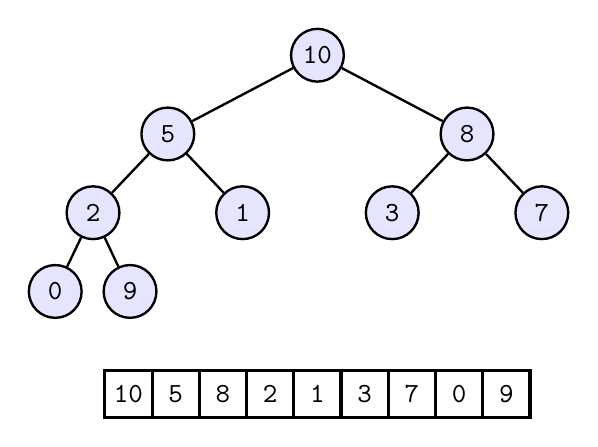
\begin{tikzpicture}

\fill[blue!10] (0.0, 0.0) circle (0.35);
\node [line width=0.03cm,black,minimum size=0.6699999999999999cm,draw,circle] at (0.0,0.0)(10){};\draw (0.0, 0.0) node[color=black] {\texttt{10}};
\fill[blue!10] (-1.9, -1.0) circle (0.35);
\node [line width=0.03cm,black,minimum size=0.6699999999999999cm,draw,circle] at (-1.9,-1.0)(5){};\draw (-1.9, -1.0) node[color=black] {\texttt{5}};
\fill[blue!10] (1.9, -1.0) circle (0.35);
\node [line width=0.03cm,black,minimum size=0.6699999999999999cm,draw,circle] at (1.9,-1.0)(8){};\draw (1.9, -1.0) node[color=black] {\texttt{8}};
\fill[blue!10] (-2.85, -2.0) circle (0.35);
\node [line width=0.03cm,black,minimum size=0.6699999999999999cm,draw,circle] at (-2.85,-2.0)(2){};\draw (-2.85, -2.0) node[color=black] {\texttt{2}};
\fill[blue!10] (-0.95, -2.0) circle (0.35);
\node [line width=0.03cm,black,minimum size=0.6699999999999999cm,draw,circle] at (-0.95,-2.0)(1){};\draw (-0.95, -2.0) node[color=black] {\texttt{1}};
\fill[blue!10] (0.95, -2.0) circle (0.35);
\node [line width=0.03cm,black,minimum size=0.6699999999999999cm,draw,circle] at (0.95,-2.0)(3){};\draw (0.95, -2.0) node[color=black] {\texttt{3}};
\fill[blue!10] (2.85, -2.0) circle (0.35);
\node [line width=0.03cm,black,minimum size=0.6699999999999999cm,draw,circle] at (2.85,-2.0)(7){};\draw (2.85, -2.0) node[color=black] {\texttt{7}};
\fill[blue!10] (-3.33, -3.0) circle (0.35);
\node [line width=0.03cm,black,minimum size=0.6699999999999999cm,draw,circle] at (-3.33,-3.0)(0){};\draw (-3.33, -3.0) node[color=black] {\texttt{0}};
\fill[blue!10] (-2.38, -3.0) circle (0.35);
\node [line width=0.03cm,black,minimum size=0.6699999999999999cm,draw,circle] at (-2.38,-3.0)(9){};\draw (-2.38, -3.0) node[color=black] {\texttt{9}};\draw[line width=0.03cm,black] (10) to  (5);
\draw[line width=0.03cm,black] (10) to  (8);
\draw[line width=0.03cm,black] (5) to  (2);
\draw[line width=0.03cm,black] (5) to  (1);
\draw[line width=0.03cm,black] (8) to  (3);
\draw[line width=0.03cm,black] (8) to  (7);
\draw[line width=0.03cm,black] (2) to  (0);
\draw[line width=0.03cm,black] (2) to  (9);

\draw (-2.3999999999999995, -4.299999999999999)
  node[draw, line width=0.04cm, , color=black,
       rounded corners=0cm, inner sep=0cm] {

\begin{minipage}[t][0.6cm]{0.6cm}
\mbox{}

\end{minipage}

};\draw (-2.3999999999999995, -4.299999999999999) node[color=black] {{\texttt{10}}};
\draw (-1.7999999999999996, -4.299999999999999)
  node[draw, line width=0.04cm, , color=black,
       rounded corners=0cm, inner sep=0cm] {

\begin{minipage}[t][0.6cm]{0.6cm}
\mbox{}

\end{minipage}

};\draw (-1.7999999999999996, -4.299999999999999) node[color=black] {{\texttt{5}}};
\draw (-1.1999999999999997, -4.299999999999999)
  node[draw, line width=0.04cm, , color=black,
       rounded corners=0cm, inner sep=0cm] {

\begin{minipage}[t][0.6cm]{0.6cm}
\mbox{}

\end{minipage}

};\draw (-1.1999999999999997, -4.299999999999999) node[color=black] {{\texttt{8}}};
\draw (-0.5999999999999996, -4.299999999999999)
  node[draw, line width=0.04cm, , color=black,
       rounded corners=0cm, inner sep=0cm] {

\begin{minipage}[t][0.6cm]{0.6cm}
\mbox{}

\end{minipage}

};\draw (-0.5999999999999996, -4.299999999999999) node[color=black] {{\texttt{2}}};
\draw (4.440892098500626e-16, -4.299999999999999)
  node[draw, line width=0.04cm, , color=black,
       rounded corners=0cm, inner sep=0cm] {

\begin{minipage}[t][0.6cm]{0.6cm}
\mbox{}

\end{minipage}

};\draw (4.440892098500626e-16, -4.299999999999999) node[color=black] {{\texttt{1}}};
\draw (0.6000000000000005, -4.299999999999999)
  node[draw, line width=0.04cm, , color=black,
       rounded corners=0cm, inner sep=0cm] {

\begin{minipage}[t][0.6cm]{0.6cm}
\mbox{}

\end{minipage}

};\draw (0.6000000000000005, -4.299999999999999) node[color=black] {{\texttt{3}}};
\draw (1.2000000000000006, -4.299999999999999)
  node[draw, line width=0.04cm, , color=black,
       rounded corners=0cm, inner sep=0cm] {

\begin{minipage}[t][0.6cm]{0.6cm}
\mbox{}

\end{minipage}

};\draw (1.2000000000000006, -4.299999999999999) node[color=black] {{\texttt{7}}};
\draw (1.8000000000000007, -4.299999999999999)
  node[draw, line width=0.04cm, , color=black,
       rounded corners=0cm, inner sep=0cm] {

\begin{minipage}[t][0.6cm]{0.6cm}
\mbox{}

\end{minipage}

};\draw (1.8000000000000007, -4.299999999999999) node[color=black] {{\texttt{0}}};
\draw (2.4000000000000004, -4.299999999999999)
  node[draw, line width=0.04cm, , color=black,
       rounded corners=0cm, inner sep=0cm] {

\begin{minipage}[t][0.6cm]{0.6cm}
\mbox{}

\end{minipage}

};\draw (2.4000000000000004, -4.299999999999999) node[color=black] {{\texttt{9}}};
\end{tikzpicture}

\end{center}


from latextool_basic import *
print(automata(layout="""
A  B  C
""",
edges="A,$a$,A|A,$b$,B|B,$a$,A|B,$b$,C|C,$a,b$,C",
A="initial|label=$q_0$",
B="label=$q_1$",
C="accept|label=$q_2$",
))
\end{python}
Of course $Q \times \Sigma^*$ is infinite so you can't
draw the whole graph!
Just include $(q, x)$ for all $x$ with length $\leq 4$.
After that draw the relation for $\vdash^*$.
\qed
\end{ex}



\newpage
You can also define acceptance using an \lq\lq extension'' of $\delta$.
Note that the transition function basically defines one single
edge (transition) in the state diagram because the second input is a
character.
There is an obvious extension to $\delta$ so that the second
input is a string:

\begin{defn}
It is convenient to extend the transition function $\delta$ so that
we allow strings for the second argument instead of just character.
Define
\[
 \delta^* : Q \times \Sigma^* \rightarrow Q
\]
\begin{itemize}
 \item[(a)] $\delta^*(q, \ep) = q$ for all $q \in Q$
 \item[(b)] $\delta^*(q, ax) = \delta^*( \delta(a,q), x)$ for $a \in
 \Sigma$, $x \in \Sigma^*$, $q \in Q$.
\end{itemize}
\end{defn}


\begin{eg} Consider this DFA again:
%-*-latex-*-

\begin{center}
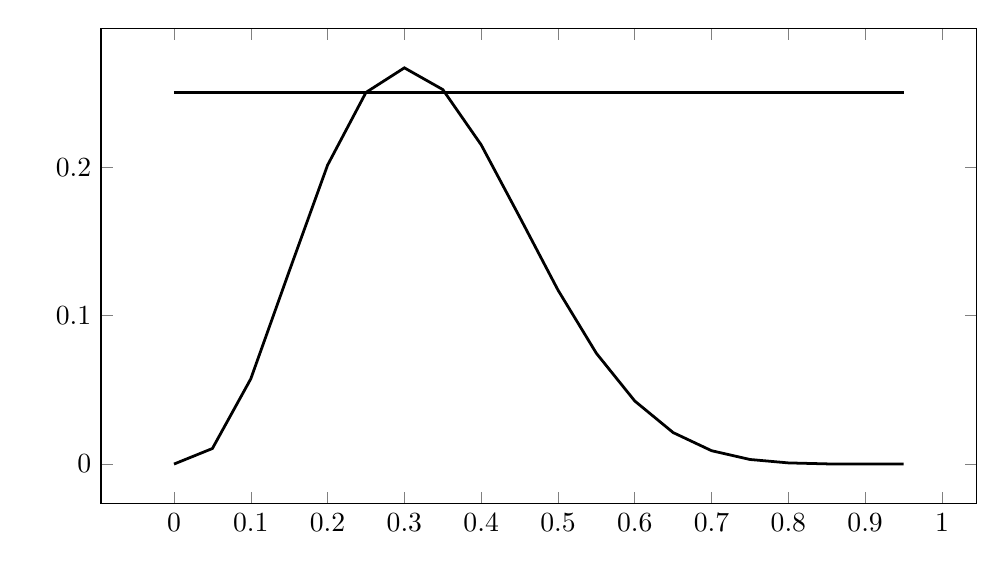
\begin{tikzpicture}[line width=1]
\begin{axis}[width=5in, height=3in,
             scatter/classes={a={mark=*,draw=black}},
             xlabel={\mbox{}},
             xlabel style={name=xlabel}, 
             ylabel={\mbox{}}, 
             legend style={
                at={(xlabel.south)},
                yshift=-1ex,
                anchor=north,
                legend cell align=left,
                },
        ]
]
\addplot[draw=black, line width=1] coordinates {(0.0, 0.0)
(0.05, 0.010475059441406248)
(0.1, 0.05739562800000002)
(0.15, 0.1298337207539062)
(0.2, 0.2013265920000001)
(0.25, 0.25028228759765625)
(0.3, 0.2668279319999998)
(0.35, 0.25221962497265626)
(0.4, 0.21499084799999998)
(0.45, 0.1664782928789064)
(0.5, 0.1171875)
(0.55, 0.07460310631640622)
(0.6, 0.042467328000000006)
(0.65, 0.02120301528515624)
(0.7, 0.009001692000000007)
(0.75, 0.00308990478515625)
(0.8, 0.000786431999999999)
(0.85, 0.0001259148164062501)
(0.9, 8.747999999999988e-06)
(0.95, 8.037890625000049e-08)};\addplot[draw=black, line width=1] coordinates {(0.0, 0.25)
(0.05, 0.25)
(0.1, 0.25)
(0.15, 0.25)
(0.2, 0.25)
(0.25, 0.25)
(0.3, 0.25)
(0.35, 0.25)
(0.4, 0.25)
(0.45, 0.25)
(0.5, 0.25)
(0.55, 0.25)
(0.6, 0.25)
(0.65, 0.25)
(0.7, 0.25)
(0.75, 0.25)
(0.8, 0.25)
(0.85, 0.25)
(0.9, 0.25)
(0.95, 0.25)};
\end{axis}\end{tikzpicture}\end{center}

from latextool_basic import *
print(automata(layout="""
A  B  C
""",
edges="A,$a$,A|A,$b$,B|B,$a$,A|B,$b$,C|C,$a,b$,C",
A="initial|label=$q_0$",
B="label=$q_1$",
C="accept|label=$q_2$",
))
  \end{python}
  Write down the $\delta^*$
  computation for $aba$. Is $aba$ accepted by the DFA?
  \end{eg}

  \SOLUTION
  Teh $\delta*$ computation is
  \begin{align*}
    \delta^*(q_0 aba)
    &= (\delta(q_0, a), ba) = (q_0, ba) \\
    &= (\delta(q_0, b), a) = (q_1, a) \\
    &= (\delta(q_1, a), \ep) = (q_0, \ep)
  \end{align*}
  I stop at this point since the string now is $\ep$.
  The last state is $q_0$ which is not an accept state.
  Therefore
  $aba$ is not accepted by the DFA.

  Comparing the above to
    \begin{align*}
    q_0 aba
    \vdash \delta(q_0, a), ba) = (q_0, ba) \\ 
    \vdash \delta(q_0, b), a) = (q_1, a) \\
    \vdash \delta(q_1, a), \ep) = (q_0, \ep)
  \end{align*}
    you see that using $\vdash$ notation to relate
    ID is mathematically the same as
    using $\delta$.
    \qed
  
Now we can define the \textit{whole} language accepted by $M$:

\begin{defn} Let $M$ be a DFA. Then the \defone{language} accepted by $M$,
denoted $L(M)$, is the language of strings over $\Sigma$ accepted
by $M$, i.e.,
\[
L(M) = \{x \in \Sigma^* \mid (q_0, x) \vdash^* (q, \ep) \text{ where } q \in F \}
\]
or
\[
L(M) = \{x \in \Sigma^* \mid \delta^* (q_0, x) \in F \}
\]
\end{defn}

\begin{ex}
\begin{tightlist}
\item Draw DFA $M$ over $\Sigma = \{0\}$ such that $L(M) = \{\}$.
\item Next, define this DFA formally.
\item Now, draw a graph where the nodes are $(q, x)$ where
$q$ runs through all the states of your DFA and $x$
runs through all the words $\Sigma^*$ ... wait
that's infinite ... you can't do that.
OK ... just draw $(q, x)$ where $q$ runs over all states
and $x$ runs over all words of length $<= 5$.
Draw directed edges in the graph so that
there's an arrow from $(q,x)$ to $(q', x')$ if
$(q, x) \vdash (q', x')$, i.e., $\delta(q, x) = \delta(q', x')$.
\item Finally graph the graph as the above except that
there's an arrow from $(q, x)$ to $(q', x')$
if $(q, x) \vdash (q', x')$, i.e.,
$\delta^*(q, x) = (q', x')$.
\end{tightlist}
\qed
\end{ex}

\begin{ex}
  Do the exercise but this time for this language:
  The DFA accepts the language of strings over 
  $\Sigma = \{a, b\}$ that contains $abab$.
  \qed
\end{ex}


\newpage
Languages over $\Sigma$ of the above kind is important.
So let's give them a name: 

\begin{defn}
A language $L$ over $\Sigma$
is \defone{regular} if $L = L(M)$ where $M$ is a DFA over $\Sigma$.
We will write $\Reg_\Sigma$ for the collection of all 
regular languages over $\Sigma$.
\end{defn}

%-*-latex-*-

\begin{center}
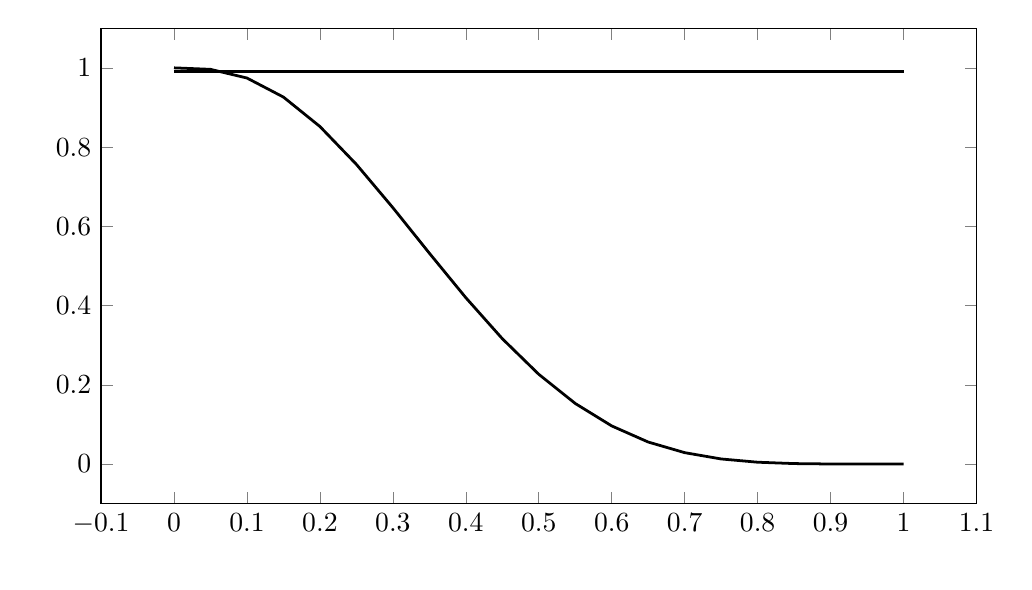
\begin{tikzpicture}[line width=1]
\begin{axis}[width=5in, height=3in,
             scatter/classes={a={mark=*,draw=black}},
             xlabel={\mbox{}},
             xlabel style={name=xlabel}, 
             ylabel={\mbox{}}, 
             legend style={
                at={(xlabel.south)},
                yshift=-1ex,
                anchor=north,
                legend cell align=left,
                },
        ]
]
\addplot[draw=black, line width=1] coordinates {(0.0, 1.0)
(0.05, 0.9962429570312497)
(0.1, 0.9743085000000002)
(0.15, 0.9262348398437498)
(0.2, 0.8519680000000004)
(0.25, 0.75640869140625)
(0.3, 0.6470694999999997)
(0.35, 0.53228332421875)
(0.4, 0.41990399999999994)
(0.45, 0.31644005078125015)
(0.5, 0.2265625)
(0.55, 0.15292768359374995)
(0.6, 0.09625600000000004)
(0.65, 0.055607535156249985)
(0.7, 0.02879550000000002)
(0.75, 0.01287841796875)
(0.8, 0.004671999999999996)
(0.85, 0.0012216445312500006)
(0.9, 0.00017649999999999982)
(0.95, 6.0273437500000275e-06)
(1.0, 0.0)};\addplot[draw=black, line width=1] coordinates {(0.0, 0.99)
(0.05, 0.99)
(0.1, 0.99)
(0.15, 0.99)
(0.2, 0.99)
(0.25, 0.99)
(0.3, 0.99)
(0.35, 0.99)
(0.4, 0.99)
(0.45, 0.99)
(0.5, 0.99)
(0.55, 0.99)
(0.6, 0.99)
(0.65, 0.99)
(0.7, 0.99)
(0.75, 0.99)
(0.8, 0.99)
(0.85, 0.99)
(0.9, 0.99)
(0.95, 0.99)
(1.0, 0.99)};
\end{axis}\end{tikzpicture}\end{center}

from latextool_basic import *

p = Plot()
r0 = Rect(0, 0, 2, 2)
x,y = r0.top()
y += 0.25
t0 = Rect(x, y, x, y, label=r'$\DFA_\Sigma$', linewidth=0)
p += r0
p += t0

r1 = Rect(4, 0, 8, 4)
x,y = r1.top()
y += 0.25
t1 = Rect(x, y, x, y, label=r'$\LANG_\Sigma$', linewidth=0)
p += r1
p += t1

r2 = Rect(4, 0, 5.5, 1.5, background='black!10')
p += r2
x,y = r2.top()
y += 0.25
t2 = Rect(x, y, x, y, label=r'$\Reg_\Sigma$', linewidth=0)
p += t2


x0,y0 = r0.right()
x1,y1 = r1.left()
p += Line(points=[(x0,y0), (x1,y0)], endstyle='>')

print(p)
\end{python}
